\section{Profilage}

Dans cette partie, nous allons mesurer et essayer d'interpréter l'impact de 
l'exécution d'une tâche \textit{best effort} sur une application temps-réel.
La tâche \textit{best effort} sera l'application Routino dans ses versions
monothread et multithread, et les tâches temps-réel seront les applications de
la suite de benchmark MiBench\cite{guthaus_mibench:_2001}. Ces mesures seront
séparées en deux parties : une analyse de l'impact sur le temps d'exécution
suivie d'une analyse de l'impact sur la bande passante. Nous essayerons ensuite
de corréler ces deux analyses.

\subsection{Analyse temporelle}
Afin d'analyser l'impact sur le temps d'exécution de la tâche temps-réel, nous
avons d'abord considérer chaque application temps-réel individuellement, puis
l'ensemble des applications comme une unique tâche, afin d'avoir un échantillon
plus important. Pour ces deux jeux de mesures, nous avons mesuré la durée 
d'exécution de la tâche temps-réel s'exécutant en isolation sur le système,
puis en concurrence avec trois instances de Routino monothread occupant
chacune un coeur, et enfin en concurrence avec un Routino multithread utilisant
trois threads effectuant les calculs. Nous calculons ensuite le surcoût en
termes de temps d'exécution par rapport à l'exécution seule de la tâche
temps-réel (Table \ref{timebench}). Il faut noter que
dans le cas où les tâches temps-réel sont analysées individuellement, les 
instances de Routinos concurrentes sont lancées en même temps que la tâche 
temps-réel et stoppées dès la fin de cette dernière. Les mesures sont ainsi
comparables, puisque chaque tâche aura été confrontée à une partie similaire 
de l'exécution de Routino.

\begin{table}[h]
\centering
\begin{tabular}{l|c|c|c|c|c}
Tâche & Temps moyen & \multicolumn{2}{c|}{Avec 3 Routinos} & 
\multicolumn{2}{c}{Avec Routino MT} \\
 & seule & Temps & Surcoût & Temps & Surcoût\\
\hline
susan\_c & 25.1 & 26.5 & 5.75\%  & 28.3 & 12.87\%\\
susan\_e & 57.2 & 58.2 & 1.60\%  & 59.4 & 3.85\%\\
fft      & 3.1  & 3.6  & 15.51\% & 3.7  & 18.64\%\\
fft\_i   & 9.3  & 10.7 & 14.72\% & 11.2 & 20.75\%\\
aes\_e   & 42.2 & 43.2 & 2.18\%  & 44.1 & 4.31\%\\
aes\_d   & 41.7 & 43.3 & 3.71\%  & 43.3 & 3.71\%\\
qsort    & 27.5 & 30.7 & 11.87\% & 32.2 & 17.14\%\\
patricia & 58.2 & 64.3 & 10.54\% & 64.5 & 10.87\%\\
\hline
Toutes   & 264.8 & 278.4 & 5.13\%  & 283.8 & 7.16\%\\
\end{tabular}
\caption{Temps d'exécution en isolation puis en concurrence (en ms) et surcoût}
\label{timebench}
\end{table}

\paragraph{}
On remarque que dans plus de la moitié des cas, le surcoût dépasse les 10\%, ce
qui pose problème pour des tâches supposées s'exécuter en temps-réel. La tâche
\textit{best effort}, à savoir Routino, a donc un impact conséquent sur le bon
fonctionnement du système. De manière plus concrète, cela signifie que le 
calcul d'itinéraire du GPS pourrait retarder la prise d'information du radar
de régulation de distance, et causer un danger pour les passagers du véhicule.

\subsection{Analyse de bande passante}
Nous allons maintenant mesurer la bande passante utilisée lors de ces
exécutions, en reprenant le même protocole que pour les mesures de temps. Les
résultats obtenus (Figure \ref{bandwidth}) seront comparées aux
mesures réalisées par Blin et al. \cite{blin_protecting_2015} et qui ont
conduit à ce projet (approximations en Table \ref{measures}).

\begin{figure}
\centering
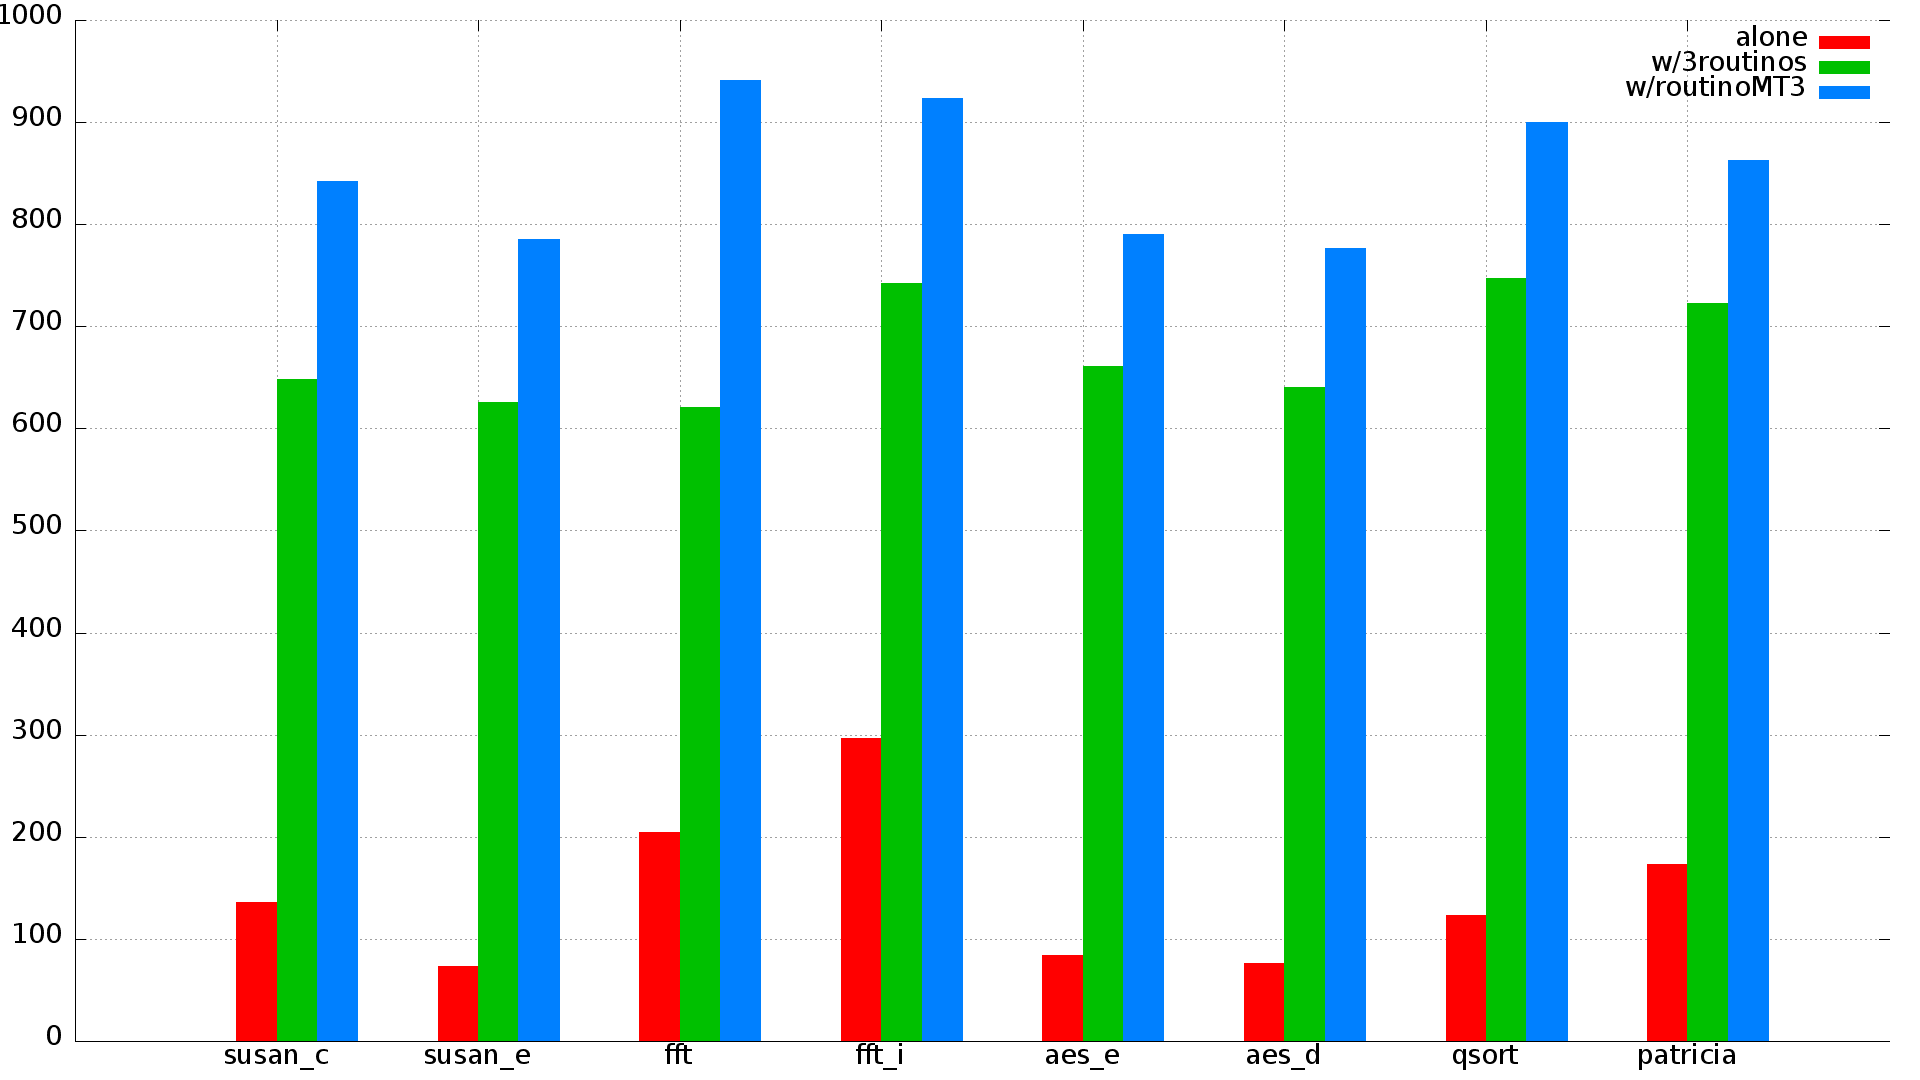
\includegraphics[scale=0.3]{include/bandwidth.png}
\caption{Utilisation moyenne de la bande passante lors des exécutions du
 MiBench (en Mo/s)}
\label{bandwidth}
\end{figure}

\begin{table}[H]
\centering
\begin{tabular}{l|c}
Tâche & Besoins bande passante (Mo/s)\\
\hline
susan\_c & 750\\
susan\_e & 600\\
fft      & 200\\
fft\_i   & 250\\
aes\_e   & 450\\
aes\_d   & 350\\
qsort    & 600\\
patricia & 500\\
\end{tabular}
\caption{Profils mémoire des tâches temps-réel}
\label{measures}
\end{table}

\paragraph{}
En nous basant sur les profils mémoire (Table \ref{measures}), les
mesures d'utilisation de bande passante (Figure \ref{bandwidth}) et sur la
caractérisation du système réalisée par Blin et al.\cite{blin_protecting_2015},
nous dressons la table \ref{carac} donnant les surcoûts que nous devrions
observer, ainsi que les surcoûts observés pour le Routino multithread.

\begin{table}[H]
\centering
\begin{tabular}{l|c|c}
Tâche & Caractérisation & Mesures\\
\hline
susan\_c & ~20\% & 12.87\%\\
susan\_e & ~5\%  & 3.85\%\\
fft      & ~2\%  & 18.64\%\\
fft\_i   & ~2\%  & 20.75\%\\
aes\_e   & ~5\%  & 4.31\% \\
aes\_d   & ~2.5\%& 3.71\%\\
qsort    & ~20\% & 17.14\%\\
patricia & ~10\% & 10.87\%\\
\end{tabular}
\caption{Surcoûts selon caractérisation du système et surcoûts mesurés}
\label{carac}
\end{table}
